\section{ODBC和JDBC}

\subsection{ODBC}

1.概念与定位

\begin{itemize}
    \item ODBC(开放数据库互连)是一套由微软发起并被各大数据库厂商支持的 C API 标准,旨在为应用程序和各种关系数据库服务器之间提供统一、与具体 DBMS 无关的连接方式。
    \item 它不需要预编译,也不特定于某一个数据库。常见的 GUI 应用、电子表格、报表工具、脚本程序等都可以通过 ODBC 驱动访问任意支持 ODBC 的后端。
\end{itemize}

2.架构与组件

\begin{itemize}
    \item ODBC 驱动管理器(Driver Manager):驻留在客户端,负责加载不同数据库厂商提供的 ODBC 驱动并转发 API 调用。
    \item ODBC 驱动(Driver):每个数据库(Oracle、SQL Server、MySQL、PostgreSQL 等)都提供相应驱动,实现标准 ODBC 接口并与其本地客户端库对接。
    \item 数据源名称(DSN, Data Source Name):在操作系统的“ODBC 数据源管理器”里预先配置,记录数据库类型、服务器地址、端口、库名、用户名、密码等连接信息。应用只需引用 DSN 即可连向对应数据库。
\end{itemize}

\begin{lstlisting}[style=cppstyle]
    SQLHENV henv;
    SQLAllocEnv(&henv);
    
    SQLHDBC hdbc;
    SQLAllocConnect(henv, &hdbc);

    SQLConnect(hdbc,
               "MyDSN", SQL_NTS,    
               "user",  SQL_NTS,   
               "pwd",   SQL_NTS);  
    
    SQLHSTMT hstmt;
    SQLAllocStmt(hdbc, &hstmt);
    
    SQLExecDirect(hstmt,
                  "SELECT branch_name, SUM(balance) FROM account GROUP BY branch_name",
                  SQL_NTS);

    SQLPrepare(hstmt, "UPDATE account SET balance = balance + ? WHERE account_number = ?", SQL_NTS);

    SQLExecute(hstmt);

    char branch[30];
    double bal;
    SQLBindCol(hstmt, 1, SQL_C_CHAR, branch, sizeof(branch), NULL);
    SQLBindCol(hstmt, 2, SQL_C_DOUBLE, &bal, 0, NULL);
    
    while (SQLFetch(hstmt) == SQL_SUCCESS) {
        printf();
    }

    SQLFreeStmt(hstmt, SQL_DROP);
    SQLDisconnect(hdbc);
    SQLFreeConnect(hdbc);
    SQLFreeEnv(henv);        
\end{lstlisting}

\subsection{IDBC}

1.概念与定位

\begin{itemize}
    \item JDBC 是 Java 平台下访问关系数据库的官方 API 标准,定义在 java.sql 包中。与 ODBC 类似,它为 Java 应用提供统一的编程接口,后端具体数据库由相应的 JDBC 驱动 实现。
    \item JDBC 支持 查询/更新、参数化预编译语句、结果集(ResultSet)、事务控制、数据库元数据检索等功能。
\end{itemize}

2.编程模型与关键类

\begin{enumerate}
    \item 加载驱动 Class.forName("oracle.jdbc.driver.OracleDriver");或者在新版 JDBC 中可不显式加载,依赖 SPI 机制。
    \item 建立连接:
       \begin{lstlisting}[style=javastyle]
        Connection conn = DriverManager.getConnection(
            "jdbc:oracle:thin:@hostname:1521:orcl",
            "user", "password"
        );  
       \end{lstlisting}  
    \item 创建语句:Statement stmt = conn.createStatement();用于执行静态 SQL
      \begin{lstlisting}[style=javastyle]
        PreparedStatement ps = conn.prepareStatement(
             "INSERT INTO account VALUES (?, ?, ?)"
        );
        ps.setString(1, "A_9732");
        ps.setString(2, "Perryridge");
        ps.setInt(3, 1200);
      \end{lstlisting}
    \item 执行 SQL
       \begin{lstlisting}[style=javastyle]
        ResultSet rs = stmt.executeQuery(
        "SELECT branch_name, AVG(balance) FROM account GROUP BY branch_name");
        int count = stmt.executeUpdate(
            "UPDATE account SET balance = balance + 100 WHERE account_number = 'A_9732'"
        );
       \end{lstlisting}
    \item 遍历结果
       \begin{lstlisting}[style=javastyle]
        while (rs.next()) {
            String branch = rs.getString("branch_name");  
            double avgBal = rs.getDouble(2);
            System.out.printf("%s: %.2f%n", branch, avgBal);
        }        
       \end{lstlisting}
    \item 异常处理:JDBC 通过抛出 SQLException 来报告各种数据库错误,应用应在 catch 块中检查 sqlState、errorCode 等。
    \item 关闭资源:
       \begin{lstlisting}[style=javastyle]
        rs.close();
        stmt.close();
        conn.close();
       \end{lstlisting}
\end{enumerate}

\begin{figure}[H]
    \centering
    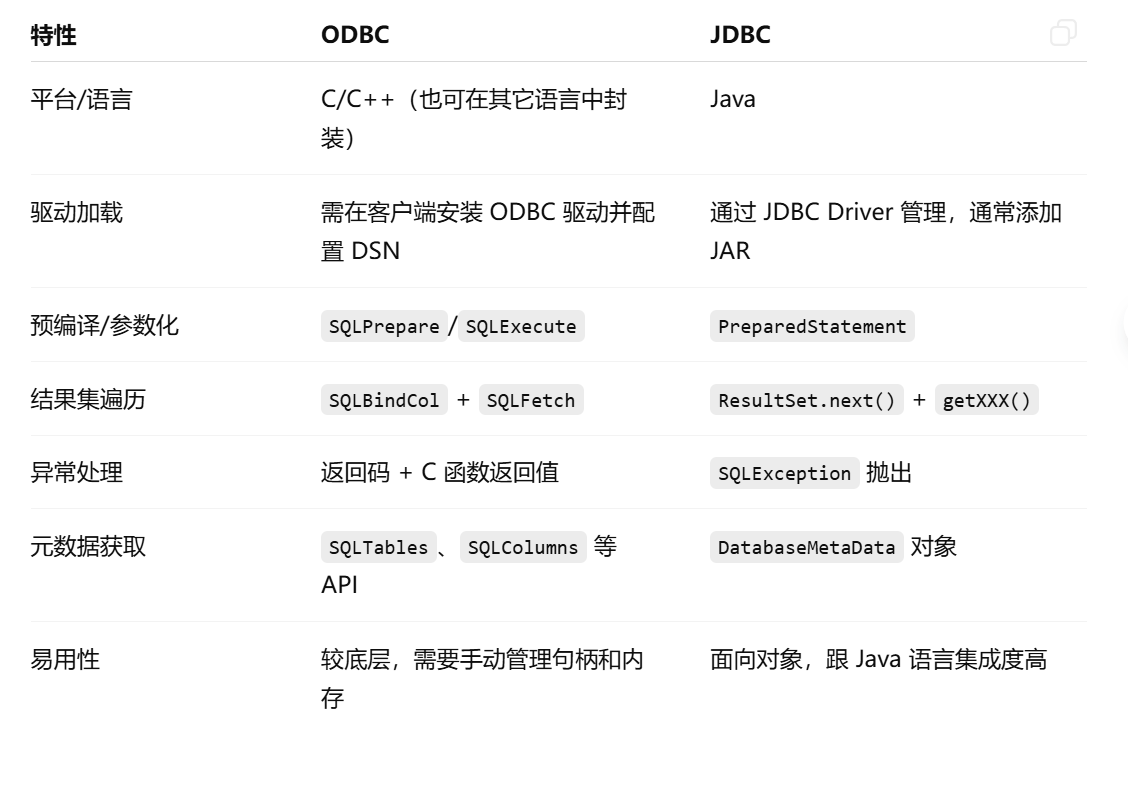
\includegraphics[width=0.8\linewidth]{image1.png}
    \caption{}
    \label{}
\end{figure}